\documentclass[12pt, spanish, pdftex]{UC3M_document}

%%%%% Preamble %%%%%
\author{Jorge Rodríguez Fraile}
\authorstwotrue
\authorsuptothree{Jorge Rodríguez Fraile}{100405951}{Grupo 83}{}{}{}{}{}{}


%%%%% Basic data about the document (Degree, subject, title, campus, page number custom text) %%%%%
\documentdata{Grado en Ingeniería Informática}{Algoritmos Genéticos y Evolutivos}{Ampliación Práctica 1 \\ Optimización de Sensores en Smart Cities}{Leganés}{}

%%%%% Page style %%%%%
\header
\footer
\pagestyle{fancy}

\begin{document}
%%%%% Page title %%%%%
\begin{titlepage}
	\centeredtitle{img/LogoUC3M.png}{\studyname}{Curso 2021-2022}{\subjectname}{\documenttitle}
	
	\begin{table}[b]
		\centering
		\begin{tabular}{ cccc }
			\large Jorge Rodríguez Fraile & \large 100405951 & \large Grupo 83 & \href{mailto:100405951@alumnos.uc3m.es}{\large 100405951@alumnos.uc3m.es} \\
			                              &                  &                 &                                                                           \\
			                              &                  &                 &                                                                           \\
		\end{tabular}
	\end{table}
	
\end{titlepage}

\newpage

%%%%% Index %%%%%
\begin{spacing}{0.5}
	% \shipout\null                   % Blank page before index (after title page)
	\hypersetup{linkcolor=black}    % References/links on the index will remain black color
	\tableofcontents\newpage        % Index of the document
	\listoffigures\newpage          % Index of pictures
	\listoftables\newpage           % Index of tables
\end{spacing}


%%%%% DOCUMENT CONTENT %%%%%
\section{Introducción}
En esta ampliación de la práctica 1 vamos a tratar de resolver el problema de las estaciones de medición de la calidad del aire de la Comunidad de Madrid mediante una nueva codificación de los individuos. Se mantienen las 24 estaciones donde cada una mide 16 variables ambientales diferentes. El problema trata sobre determinar que sensores de los presentes en las estaciones deben estar permanentemente o programados para reducir el coste de su mantenimiento e instalación, pero sin perder precisión en las mediciones.

\section{Codificación y Función de fitness}
En este caso la codificación pasará de ser binaria, cada individuo un vector de 384 bits de 0 y 1, a una codificación discreta, vector de 384 valores con 3 posibles valores cada uno, los valores que podrá tomar son:
\begin{itemize}
	\item \textbf{0:} No se instala el sensor en la estación.
	\item \textbf{F:} El sensor se instala en la estación y se usa de manera permanente.
	\item \textbf{H:} El sensor se instala en la estación, pero se programa su uso.
\end{itemize}
Cada uno de los cromosomas estará representado por $24 \cdot 16=384$ genes de manera que cada 16 valores sea una estación distinta, se empezará por el primer sensor de la primera estación, después el segundo sensor y así hasta el último de la primera para dar paso a la siguiente estación. En cuanto al sensor que representa cada valor son los siguientes:
\begin{table}[H]
	\centering
	\caption{Medidas de los sensores}
	\begin{tabular}{|l|l|l|l|}
		\hline
		1  & Dióxido de Azufre           & SO$_2$ & µg/m$^3$ \\ \hline
		2  & Monóxido de Carbono         & CO     & µg/m$^3$ \\ \hline
		3  & Monóxido de Nitrógeno       & NO     & µg/m$^3$ \\ \hline
		4  & Dióxido de Nitrógeno        & NO$_2$ & µg/m$^3$ \\ \hline
		5  & Partículas \textless 2.5 µm & PM2.5  & µg/m$^3$ \\ \hline
		6  & Partículas \textless 10 µm  & PM10   & µg/m$^3$ \\ \hline
		7  & Óxidos de Nitrógeno         & NOx    & µg/m$^3$ \\ \hline
		8  & Ozono                       & O$_3$  & µg/m$^3$ \\ \hline
		9  & Tolueno                     & TOL    & µg/m$^3$ \\ \hline
		10 & Benceno                     & BEN    & µg/m$^3$ \\ \hline
		11 & Etilbenceno                 & EBE    & µg/m$^3$ \\ \hline
		12 & Metaxileno                  & MXY    & µg/m$^3$ \\ \hline
		13 & Paraxileno                  & PXY    & µg/m$^3$ \\ \hline
		14 & Ortoxileno                  & OXY    & µg/m$^3$ \\ \hline
		15 & Hexano (total)              & TCH    & mg/m$^3$ \\ \hline
		16 & Hexano (no metánicos)       & NMHC   & mg/m$^3$ \\ \hline
	\end{tabular}
\end{table}
Ejemplo: 00F00F0H00000000 0000000000000000 … \\ Indica que en la primera estación se instalan los sensores de NO permanente, PM10 permanente y O$_3$ se programará, sin embargo en la segunda estación ni siguiera se instala al no tener sensores.

Aunque la codificación ya la hemos decidido se analizara su conveniencia para los algoritmos genéticos:
\begin{itemize}
	\item La codificación es completa, todas las posibilidades de sensores para todas las estaciones son codificables.
	\item Solo se codifican soluciones factibles.
	\item Cada solución solo tiene una posible solución.
	\item La descodificación es fácil y rápida, cada 16 valores es una estación y cada uno de esos valores un sensor.
	\item La codificación es adyacente, es decir, al variar un bit los cambios que experimenta son pequeños, se pone de manera permanente, programada o se quita un sensor de una estación.
\end{itemize}

El espacio de búsqueda se compone ahora de $3^{384}$ posibles soluciones, lo que lo hace $4,16 \cdot 10^{67}$ veces más grande que el de codificación binaria. Esto nos hace pensar que emplea algoritmos genéticos en este problema es una buena idea, ya que si no era posible por fuerza bruta en binario este mucho menos.

\section{Cambios}
Para realizar esta ampliación ha sido necesario modificar el programa que se había desarrollado, los aspectos cambiados son los que se describen en las siguientes subsecciones, el resto se mantiene igual.

\subsection{Convergencia y Fitness}
La función de fitness que se emplea para esta ampliación se obtiene mediante una petición de get a \\ \href{http://memento.evannai.inf.uc3m.es/age/alfa2?c=}{http://memento.evannai.inf.uc3m.es/age/alfa2?c=} seguido por el cromosoma que deseamos evaluar, el cambio es la web a la que consultar. Para obtener la evaluación de una población se utilizará el mismo método que en la parte anterior, \textit{evaluate\_population(population, num\_evaluations)}.

El criterio de convergencia se ha mantenido igual con respecto a la práctica base, termina si llega a 0 o si llega a una determinada generación máxima.

\subsection{Población inicial}
Se ha modificado el método \textit{initial\_population()} que en este caso en vez de generar como base una matriz de 0 con numpy genera una matriz de elementos del tipo carácter, esto nos permitirá poder almacenar los numero y letras (0, H y F). El vector generado conserva las mismas dimensiones, tantas filas como individuos y tantas columnas como genes.

Después para rellenar la matriz con nuestros individuos de manera aleatoria, lo que se ha hecho es generar un número entero entre 0 y 2 incluido. Para cada posición de la matriz se le asigna uno de los posibles valores en función del valor aleatorio que se genera, si sale 0 es 0, 1 es H y 2 es F.

\subsection{Mutación}
El operador de mutación \textit{mutation(population, factor)} ha sido necesario modificarlo dado que ya no vale que si se hace mutación de un gen se calcule como 1-valorAnterior, en este caso cuando se vaya a mutar un gen se calculará un valor entero entre 0 y 1 incluido, de esta manera se podrá elegir aleatoriamente entre los otros 2 valores para el gen.
\pagebreak

\section{Pruebas}
Los modelos se han nombrado siguiendo una codificación con el siguiente formato XX\_YY\_ZZ, tal que:
\begin{itemize}
	\item \textbf{XX:} Número de generaciones generadas.
	\item \textbf{YY:} Tamaño del conjunto de candidatos al hacer torneo para la selección.
	\item \textbf{ZZ:} Porcentaje de mutaciones sobre la población.
\end{itemize}

Las pruebas realizadas en esta ampliación corresponden con los 2 mejores modelos que se obtuvieron en la parte anterior. Se ha probado además una ampliación del mejor modelo poniéndole 2000 ciclos máximos. Los modelos probados son:
\begin{itemize}
	\item 200 ciclos máximos, 10 individuos por torneo y un porcentaje de mutación del 0,5 \%.
	\item 2000 ciclos máximos, tamaño de torneo 10 y con un porcentaje de realizar mutación del 0,5 \%.
	\item 1000 ciclos máximos, tamaño de torneo 10 y con un porcentaje de realizar mutación del 0,1 \%.
\end{itemize}

Se ha optado por añadir el de 2000 generaciones dado que cambiar los torneos o mutación empeoraba los resultados y dado que ahora hay muchas más posibles soluciones, por lo que ampliar las generaciones máximas era una buena opción para probar.

A continuación se presentan de manera gráfica los resultados obtenidos para los modelos durante 5 ejecuciones y su media en forma de línea, se ha optado por realizar 5 ejecuciones para poder ver como de buenos son los modelos y evitar el sesgo.
\begin{figure}[H]
	\ffigbox[\FBwidth]
	{\caption{Evaluación de los Modelos probados}}
	{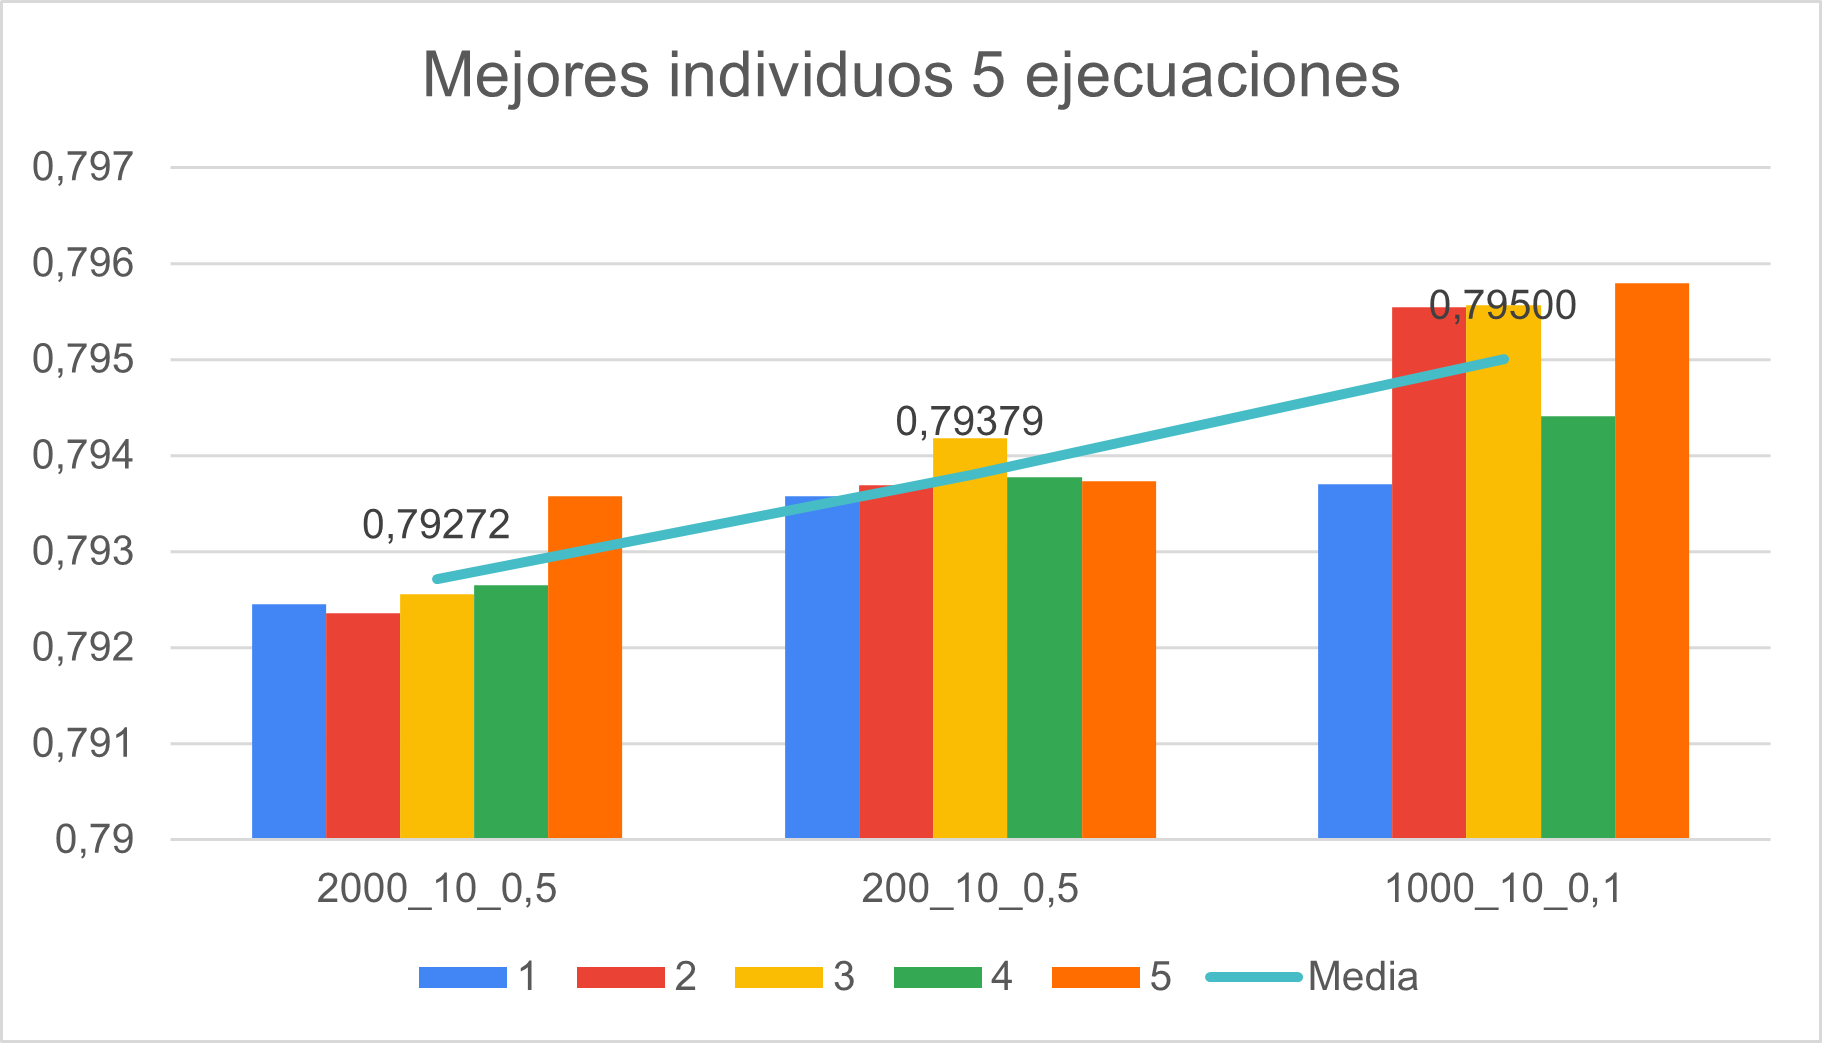
\includegraphics[scale=1]{./img/geneticAmpliation.png}}
\end{figure}
Los datos en los que se basa la gráfica son los de la siguiente tabla, en la que se ha marcado para cada uno de los modelos cuál es la mejor prueba en una escala de verde a rojo, siendo verde el mejor y rojo el peor. Se ha elegido el gradiente para cada modelo y no en general para facilitar la distinción de los tonos de colores. Además, se presenta la media de las pruebas, también siguiendo el gradiente de color verde a rojo.
\begin{table}[H]
	\centering
	\caption{Fitness primeros modelos}
	\resizebox{\textwidth}{!}{%
	\begin{tabular}{|l|l|l|l|l|l|l|}
		\hline
		\rowcolor[HTML]{4285F4} 
		\multicolumn{1}{|c|}{\cellcolor[HTML]{4285F4}{\color[HTML]{FFFFFF} \textbf{Modelo}}} & \multicolumn{1}{c|}{\cellcolor[HTML]{4285F4}{\color[HTML]{FFFFFF} \textbf{1}}} & \multicolumn{1}{c|}{\cellcolor[HTML]{4285F4}{\color[HTML]{FFFFFF} \textbf{2}}} & \multicolumn{1}{c|}{\cellcolor[HTML]{4285F4}{\color[HTML]{FFFFFF} \textbf{3}}} & \multicolumn{1}{c|}{\cellcolor[HTML]{4285F4}{\color[HTML]{FFFFFF} \textbf{4}}} & \multicolumn{1}{c|}{\cellcolor[HTML]{4285F4}{\color[HTML]{FFFFFF} \textbf{5}}} & \multicolumn{1}{c|}{\cellcolor[HTML]{4285F4}{\color[HTML]{FFFFFF} \textbf{Media}}} \\ \hline
		2000\_10\_0,5 & \cellcolor[HTML]{6EC17B}0,792457154 & \cellcolor[HTML]{63BE7B}0,792358877 & \cellcolor[HTML]{7AC47C}0,792563621 & \cellcolor[HTML]{84C77C}0,792647846 & \cellcolor[HTML]{F0E683}0,793575478 & \cellcolor[HTML]{63BE7B}0,792720595 \\ \hline
		200\_10\_0,5 & \cellcolor[HTML]{F0E683}0,793575478 & \cellcolor[HTML]{FEEA83}0,793694524 & \cellcolor[HTML]{FECE7F}0,794183547 & \cellcolor[HTML]{FFE784}0,793778166 & \cellcolor[HTML]{FFE984}0,793740165 & \cellcolor[HTML]{FFEB84}0,793794376 \\ \hline
		1000\_10\_0,1 & \cellcolor[HTML]{FFEB84}0,793702786 & \cellcolor[HTML]{F9796F}0,79554339 & \cellcolor[HTML]{F9786E}0,79556596 & \cellcolor[HTML]{FDC07C}0,794407778 & \cellcolor[HTML]{F8696B}0,795797182 & \cellcolor[HTML]{F8696B}0,795003419 \\ \hline
		\end{tabular}%
	}
\end{table}
\vspace{-.5cm}
Podemos ver que en general dan buenos resultados, como pasaba en la parte anterior de la práctica el mejor modelo ha sido el correspondiente a \textbf{tamaño de torneo 10} y \textbf{porcentaje de mutación del 0,5 \%}. En la siguiente sección se explicará en más detalle la mejor solución.

\subsection{Resultado}
El mejor modelo que se ha obtenido ha sido el \textbf{2000\_10\_0,5}, que corresponde a un máximo de \textbf{2000 generaciones} que han sido \textbf{200100 evaluaciones}, aunque de media los mejores resultados han necesitado 107320 evaluaciones (1074 generaciones), con un tamaño de \textbf{torneo de 10 individuos} y un porcentaje de \textbf{mutación del 0,5 \%} de la población, el mejor resultado obtenido tiene un \textbf{fitness de 0,792358877114} y su cromosoma asociado es:

0000HHHH00H0H0H0 0H00HH0HH0H0H0H0 00H0H00H00H0000H 0H0HHHHHH000H0H0 000H0H00H0H0H0HH 0H00H0H000000HH0 0H0HH0HHHHH0H00H 00HH0HHHHH00HHH0 0H0HHH0HH0H000H0 00H0H0HH0HH000HH 0HH0H00HH0H0H000 0HHHH000H0H0HH0H 0H0HH0H00HH0H0H0 000HH000HH00H00H 0H0HH00HH0H000HH 0H0000H00000H0HH 00H0H000H0H0HHHH 0HHH0H0HHH00H0HH H000000H0H0000HH H000HH0H0HH0HHH0 0H0HH00HH0H000H0 0H0H0HHH000000HH 0H00HH00H0H0HH00 0HHH0H00H0H0H000

Algo que se puede observar en esta solución es que no hay ningún gen con valor F, los sensores no se instalan o se programan, pero no merece la pena dejarlos de manera permanente.

En la siguiente gráfica se muestra cuál ha sido la progresión del fitness a lo largo de las evaluaciones para este modelo.
\begin{figure}[H]
	\ffigbox[\FBwidth]
	{\caption{Fitness vs. Evaluaciones 1000\_10\_0,5}}
	{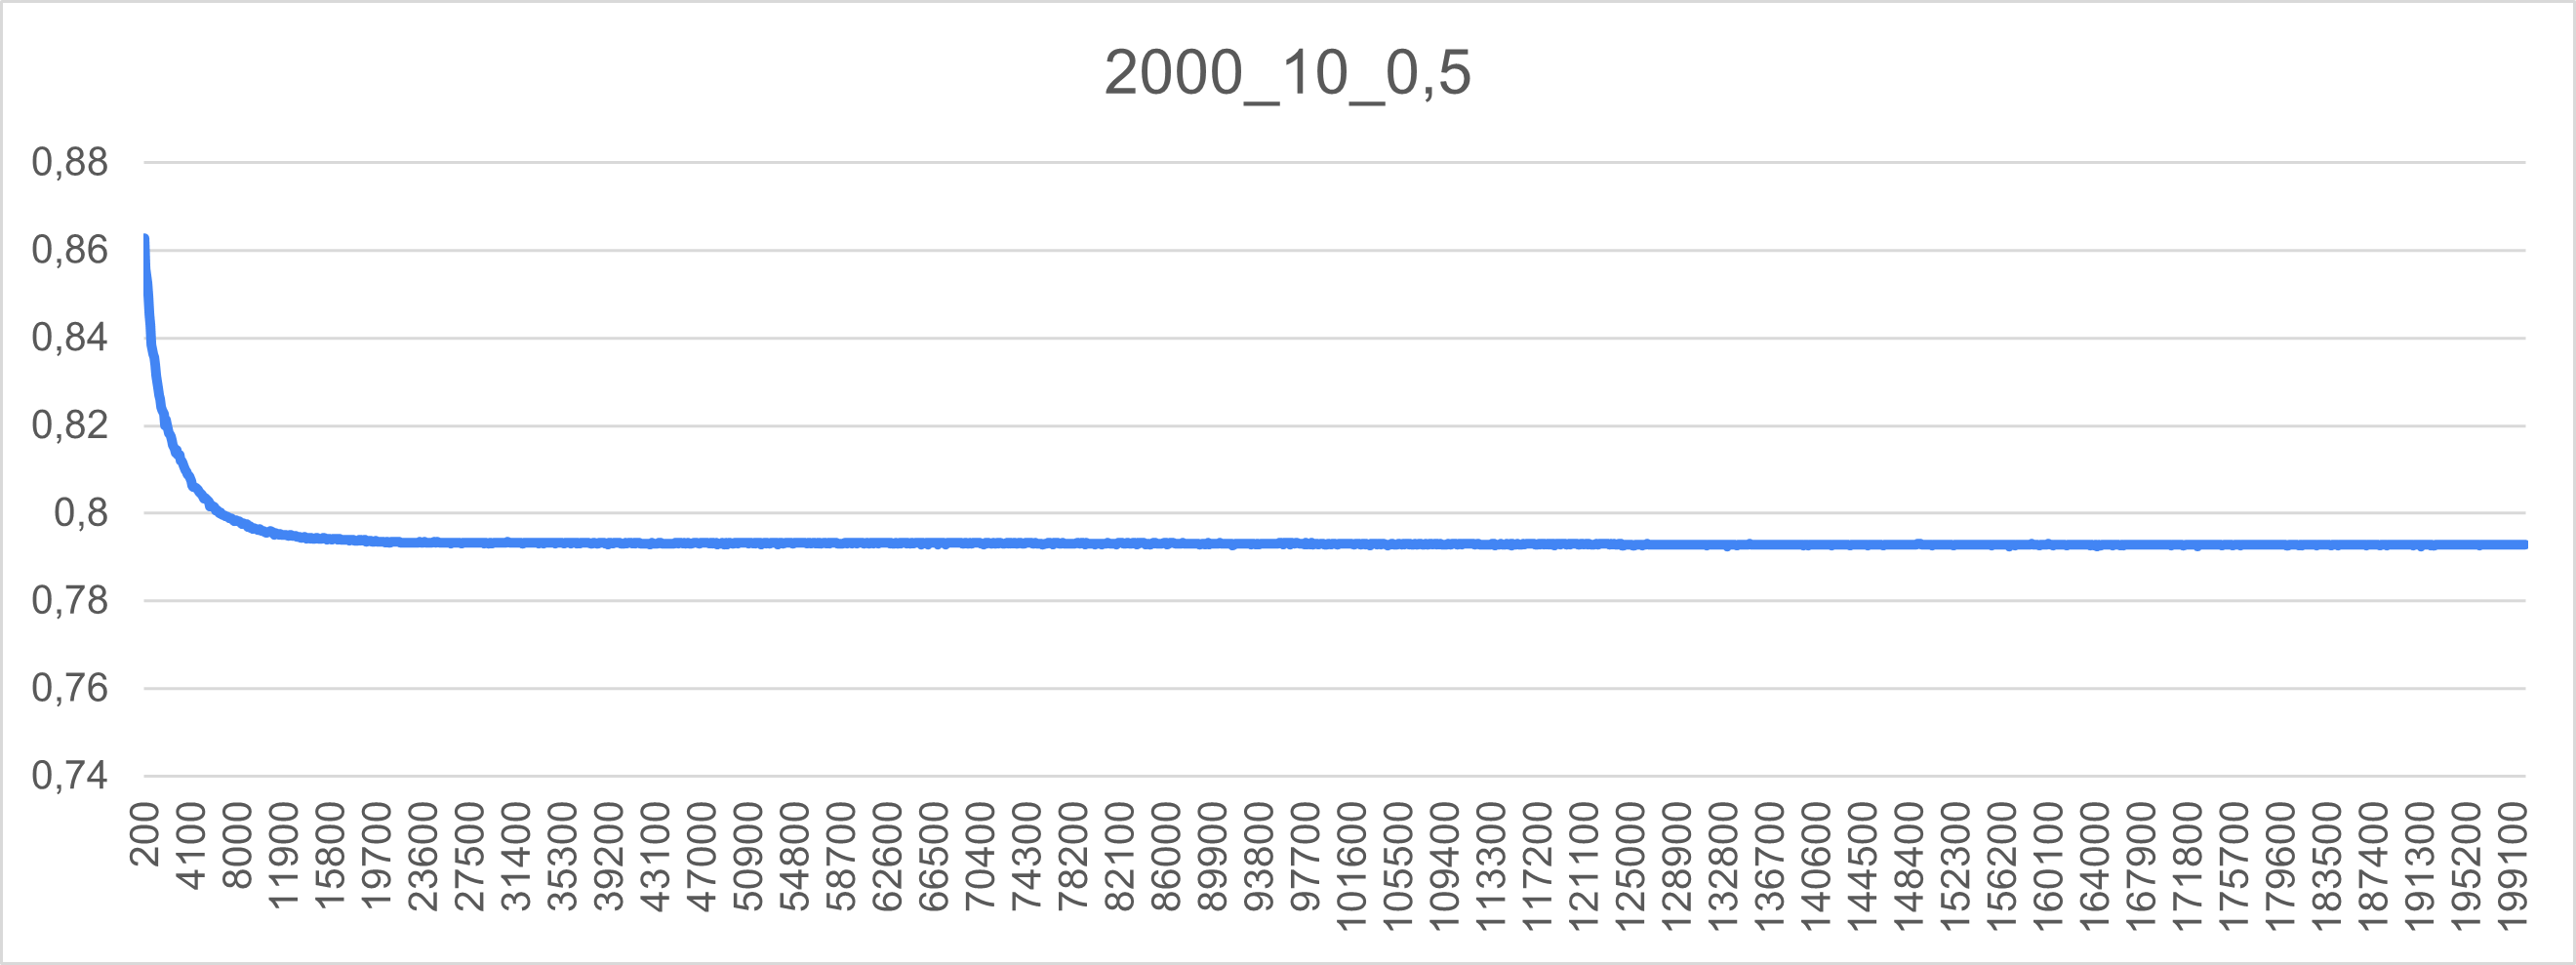
\includegraphics[scale=.8]{./img/2000_10_0,5.png}}
\end{figure}
\pagebreak

Como se puede ver el fitness al comienzo baja rápidamente y llegado un punto se empieza a estabilizar, hay subidas y bajadas mínimas, pero no hay una tendencia a mejorar o empeorar muy marcada. El mejor resultado está en la evaluación 172600, pero como se puede ver los valores llevaban muchos ciclos oscilando entre 0,793 y 0,794.

El significado del cromosoma que se ha puesto más arriba es que las estaciones tendrán los siguientes sensores programados, dado que no hay ninguno que se instale de manera permanente:
\begin{itemize}
	\item \textbf{Estación 1:} PM2.5, PM10, NOx, O$_3$, EBE, PXY y TCH.
	\item \textbf{Estación 2:} CO, PM2.5, PM10, O$_3$, TOL, EBE, PXY y TCH.
	\item \textbf{Estación 3:} NO, PM2.5, O$_3$, EBE y NMHC.
	\item \textbf{Estación 4:} CO, NO$_2$, PM2.5, PM10, NOx, O$_3$, TOL, PXY y TCH.
	\item \textbf{Estación 5:} NO$_2$, PM10, TOL, EBE, PXY, TCH y NMHC.
	\item \textbf{Estación 6:} CO, PM2.5, NOx, OXY y TCH.
	\item \textbf{Estación 7:} CO, NO$_2$, PM2.5, NOx, O$_3$, TOL, BEN, EBE, PXY y NMHC.
	\item \textbf{Estación 8:} NO, NO$_2$, PM10, NOx, O$_3$, TOL, BEN, PXY, OXY y TCH.
	\item \textbf{Estación 9:} CO, NO$_2$, PM2.5, PM10, O$_3$, TOL, EBE y TCH.
	\item \textbf{Estación 10:} NO, PM2.5, NOx, O$_3$, BEN, EBE, TCH y NMHC.
	\item \textbf{Estación 11:} CO, NO, PM2.5, O$_3$, TOL, EBE y PXY.
	\item \textbf{Estación 12:} CO, NO, NO$_2$, PM2.5, TOL, EBE, PXY, OXY y NMHC.
	\item \textbf{Estación 13:} CO, NO$_2$, PM2.5, NOx, BEN, EBE, PXY y TCH.
	\item \textbf{Estación 14:} NO$_2$, PM2.5, TOL, BEN, PXY y NMHC.
	\item \textbf{Estación 15:} CO, NO$_2$, PM2.5, O$_3$, TOL, EBE, TCH y NMHC.
	\item \textbf{Estación 16:} CO, NOx, PXY, TCH y NMHC.
	\item \textbf{Estación 17:} NO, PM2.5, TOL, EBE, PXY, OXY, TCH y NMHC.
	\item \textbf{Estación 18:} CO, NO, NO$_2$, PM10, O$_3$, TOL, BEN, PXY, TCH y NMHC.
	\item \textbf{Estación 19:} SO$_2$, O$_3$, BEN, TCH y NMHC.
	\item \textbf{Estación 20:} SO$_2$, PM2.5, PM10, O$_3$, BEN, EBE, PXY, OXY y TCH.
	\item \textbf{Estación 21:} CO, NO$_2$, PM2.5, O$_3$, TOL, EBE y TCH.
	\item \textbf{Estación 22:} CO, NO$_2$, PM10, NOx, O$_3$, TCH y NMHC.
	\item \textbf{Estación 23:} CO, PM2.5, PM10, TOL, EBE, PXY y OXY.
	\item \textbf{Estación 24:} CO, NO, NO$_2$, PM10, TOL, EBE y PXY.
\end{itemize}

\section{Conclusiones}
En este proyecto se ha abordado el problema de seleccionar sensores para estaciones de control de calidad del aire en la ciudad Madrid con una nueva codificación. Se ha podido comprobar que esta nueva codificación para el problema es viable y se obtienen buenas soluciones empleando algoritmos genéticos, cosa que no ocurriría con fuerza bruta como vimos en la práctica base. Además, que los modelos que se idearon en la práctica base siguen funcionando para esta codificación.

En cuanto a la codificación se ha podido ver que las soluciones cuando van evolucionando y mejorando nunca codifican soluciones que instalen de manera permanente sensores en las estaciones, al igual que todas las soluciones mantienen las 24 estaciones y no dejan ninguna vacía.

\end{document}